% !TEX root = Main.tex
\appendix
\appendixpage
\addappheadtotoc
\section{The benzene molecule}\label{benzex}
\begin{wrapfigure}[7]{r}{.3\textwidth}
	\vspace{-2.3em}
	\centering
	\begin{tikzpicture}
		\chemfig{1*6(-2-3-4-5-6-)}
	\end{tikzpicture}
	\caption{Indices of a benzene molecule}\label{benz}
\end{wrapfigure}
As an example the Hamiltonian of benzene is considered. In \cref{benz} one can see the indices of a benzene molecule. Remember that \(\bra{\phi_{\pi}(1)}\hat{H}\ket{\phi_{\pi}(1)} = 0\) and \cref{V}, the Hamiltonian reads:
\begin{align}
	\mqty{                            \\ \\ \\ \vb{H} = V_{pp\pi}\\ \\ \\} \ \mqty{						&  \mqty{1 & 2 & 3 & 4 & 5 & 6} \\
		\mqty{1                           \\ 2 \\ 3 \\ 4 \\ 5 \\ 6} &	\mqty*(0 & 1 & 0 & 0 & 0 & 1 \\
	1 & 0 & 1 & 0 & 0 & 0             \\
	0 & 1 & 0 & 1 & 0 & 0             \\
	0 & 0 & 1 & 0 & 1 & 0             \\
	0 & 0 & 0 & 1 & 0 & 1             \\
	1 & 0 & 0 & 0 & 1 & 0)}\label{BH}
\end{align}
As a helping aid, \cref{BH} shows the atomic indices of the atom on the top and to the left of the matrix. This will give an understanding of how to work with such matrices.
The structure of the benzene molecule is rotationally symmetric and rotating the indices one sixth must yield the same Hamiltonian. Consider the energy eigenvector:
\begin{align}
	\phi = \mqty(c_1 & c_2 & c_3 & c_4 & c_5 & c_6)
\end{align}
There must exist an operator that rotates the indices as such:
\begin{align}
	C_6\phi = \mqty(c_2 & c_3 & c_4 & c_5 & c_6 & c_1)
\end{align}
The rotated Hamiltonian is the same, and thus \(C_6\) and \(\vb{H}\) commute. The rotated vector must be an eigenvector with the same energy and it should be possible to find simultaneous eigenvectors to \(C_6\) and \(\vb{H}\).
\begin{align}
	C_6\phi = \mqty(c_2 & c_3 & c_4 & c_5 & c_6 & c_1) = \lambda\mqty(c_1 & c_2 & c_3 & c_4 & c_5 & c_6)
\end{align}
This operator \(C_6\) is represented with the matrix:
\begin{align}
	\vb{C}_6 = \mqty*(0 & 1 & 0 & 0 & 0 & 0  \\
	0                   & 0 & 1 & 0 & 0 & 0  \\
	0                   & 0 & 0 & 1 & 0 & 0  \\
	0                   & 0 & 0 & 0 & 1 & 0  \\
	0                   & 0 & 0 & 0 & 0 & 1  \\
	1                   & 0 & 0 & 0 & 0 & 0)
\end{align}
It can quickly be shown that the normalised eigenvectors to \(C_6\) are
\begin{align}
	\phi_n = \frac{1}{\sqrt{6}}\mqty(\lambda_n^0 & \lambda_n^1 & \lambda_n^2 & \lambda_n^3 & \lambda_n^4 & \lambda_n^5), \quad \lambda_n = \exp{-i2\pi n / 6}, \quad n = 0,1,2,3,4,5
\end{align}
These eigenvectors are also eigenvectors for \(\vb{H}\) with the eigenvalues:
\begin{align}
	\varepsilon_n = \lambda_n + \lambda_{n-1} = 2 \cos{n\pi/3}
\end{align}
Thus thanks to the rotational symmetry it was possible to find the eigenvectors and eigenenergies for the Hamiltonian.
\section{Additional figures}\label{appfigs}
\begin{figure}[h]
	\centering
	\begin{subfigure}[b]{0.45\textwidth}
		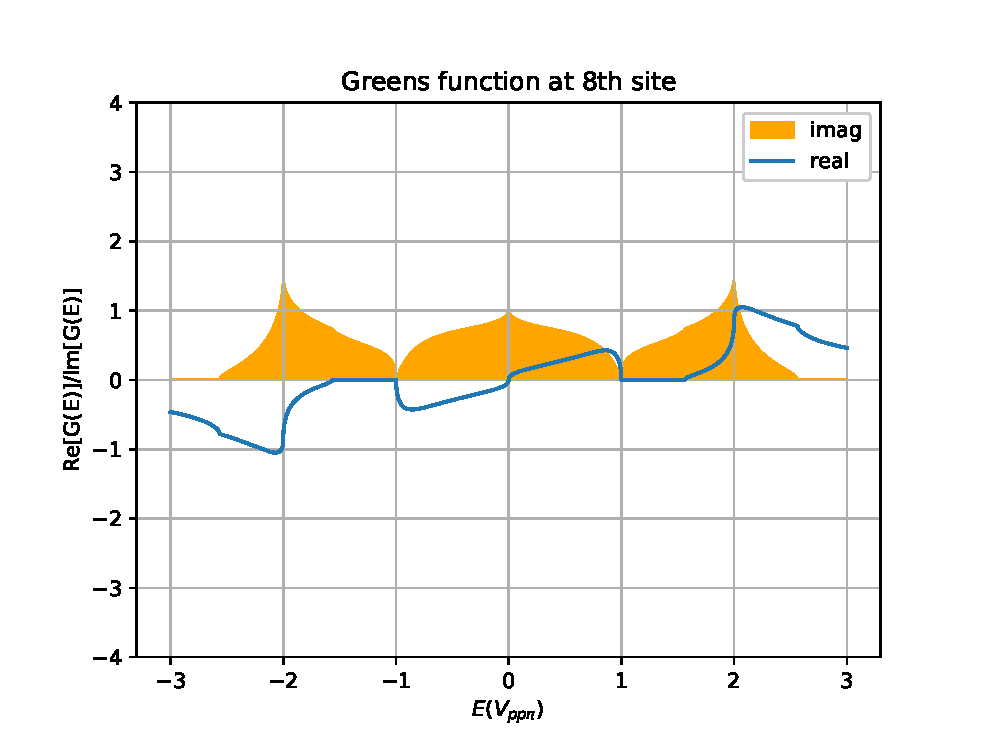
\includegraphics[width=\textwidth]{Figures/BetaimrealTE8.eps}
		\caption{Figure showing a plot of the Green's function at the \nth{8} site}
		\label{4th}
	\end{subfigure}
	~ %add desired spacing between images, e. g. ~, \quad, \qquad, \hfill etc.
	%(or a blank line to force the subfigure onto a new line)
	\begin{subfigure}[b]{0.45\textwidth}
		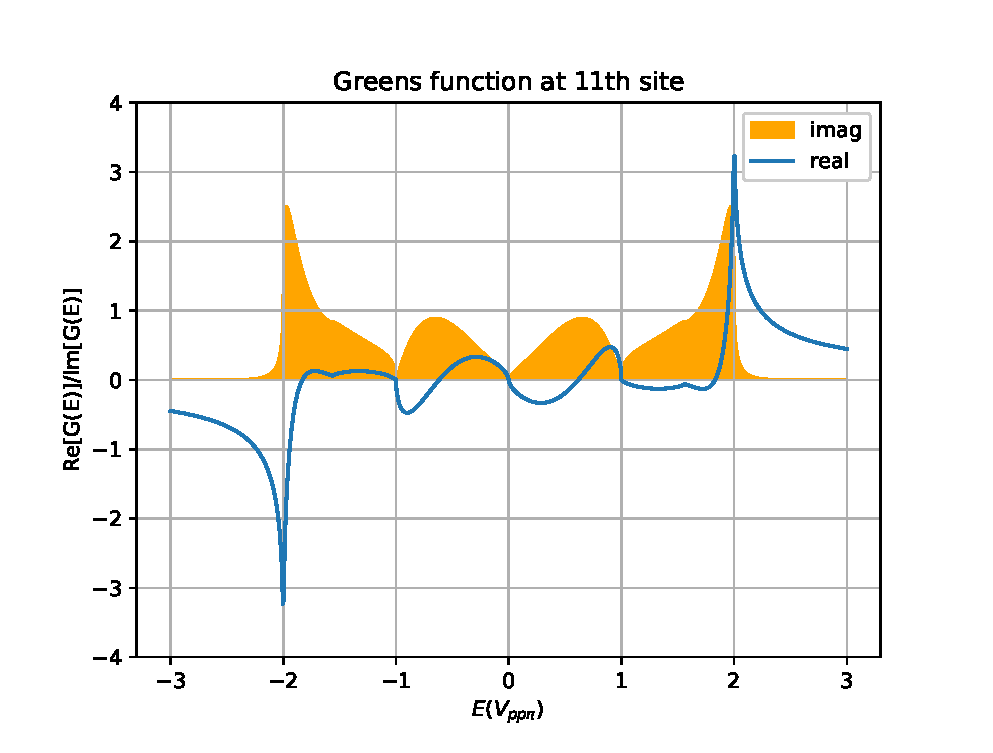
\includegraphics[width=\textwidth]{Figures/BetaimrealTE11.eps}
		\caption{Figure showing a plot of the Green's function at the \nth{11} site}
		\label{7th}
	\end{subfigure}
	\caption{Two plots showing how the Green's function changes as the site is changed. The \nth{8} and \nth{11} sites are corresponding to atoms of those indices (8, 11) in \cref{pointplot}. Note how the LDOS changes (imaginary part) for the different sites.}\label{siteLDOSplot}
\end{figure}
\begin{figure}
	\centering
	\begin{subfigure}[b]{0.3\textwidth}
		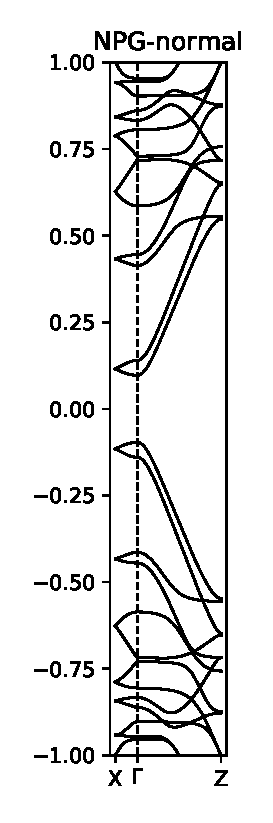
\includegraphics[width=\textwidth]{Figures/FabNPGBS.eps}
		\caption{Normal NPG}
		\label{Fabbs}
	\end{subfigure}
	~ %add desired spacing between images, e. g. ~, \quad, \qquad, \hfill etc.
	%(or a blank line to force the subfigure onto a new line)
	\begin{subfigure}[b]{0.3\textwidth}
		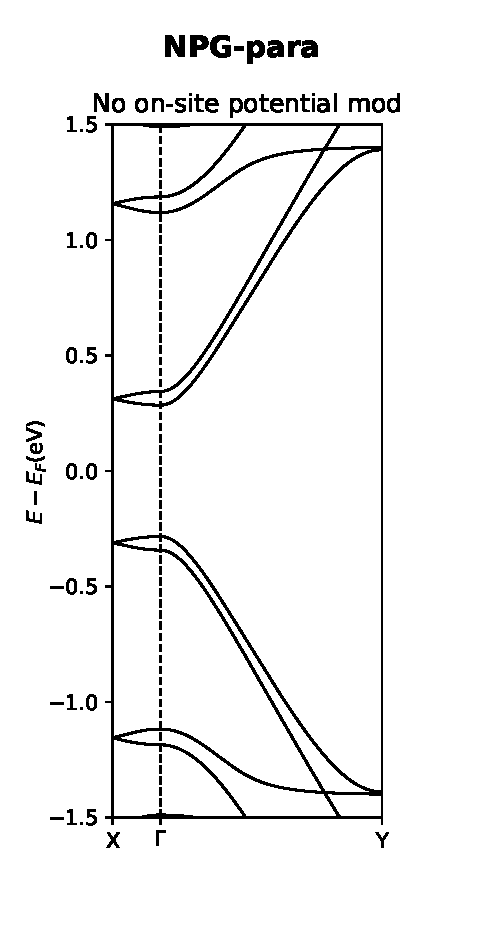
\includegraphics[width=\textwidth]{Figures/paraNPGBS.eps}
		\caption{Para NPG}
		\label{parabs}
	\end{subfigure}
	~ %add desired spacing between images, e. g. ~, \quad, \qquad, \hfill etc.
	%(or a blank line to force the subfigure onto a new line)
	\begin{subfigure}[b]{0.3\textwidth}
		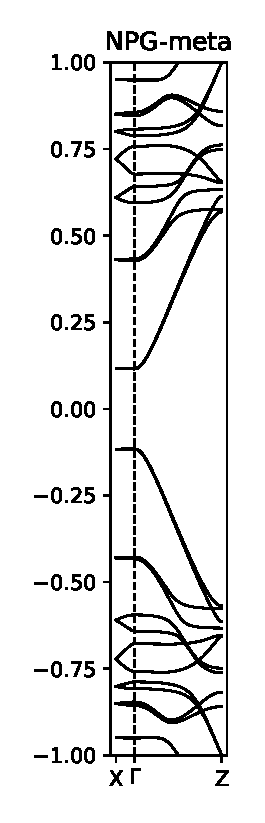
\includegraphics[width=\textwidth]{Figures/metaNPGBS.eps}
		\caption{Meta NPG}
		\label{metabs}
	\end{subfigure}
	\caption{Plot showing band structures in the energy range \SI{-1.5}{\electronvolt} to \SI{1.5}{\electronvolt} for normal, para and meta NPG. The are plotted between symmetry points \(X\) and \(Y\) with respect to the origin \(\Gamma\)}\label{allbands}
\end{figure}
\im{Listings/Functions.py}{41}{47}
\vspace{-1\baselineskip}
\captionof{listing}{Function creating the hopping matrices between two sets of coordinates \label{hopfunc}}\vspace{\baselineskip}

\begin{figure}
	\centering
	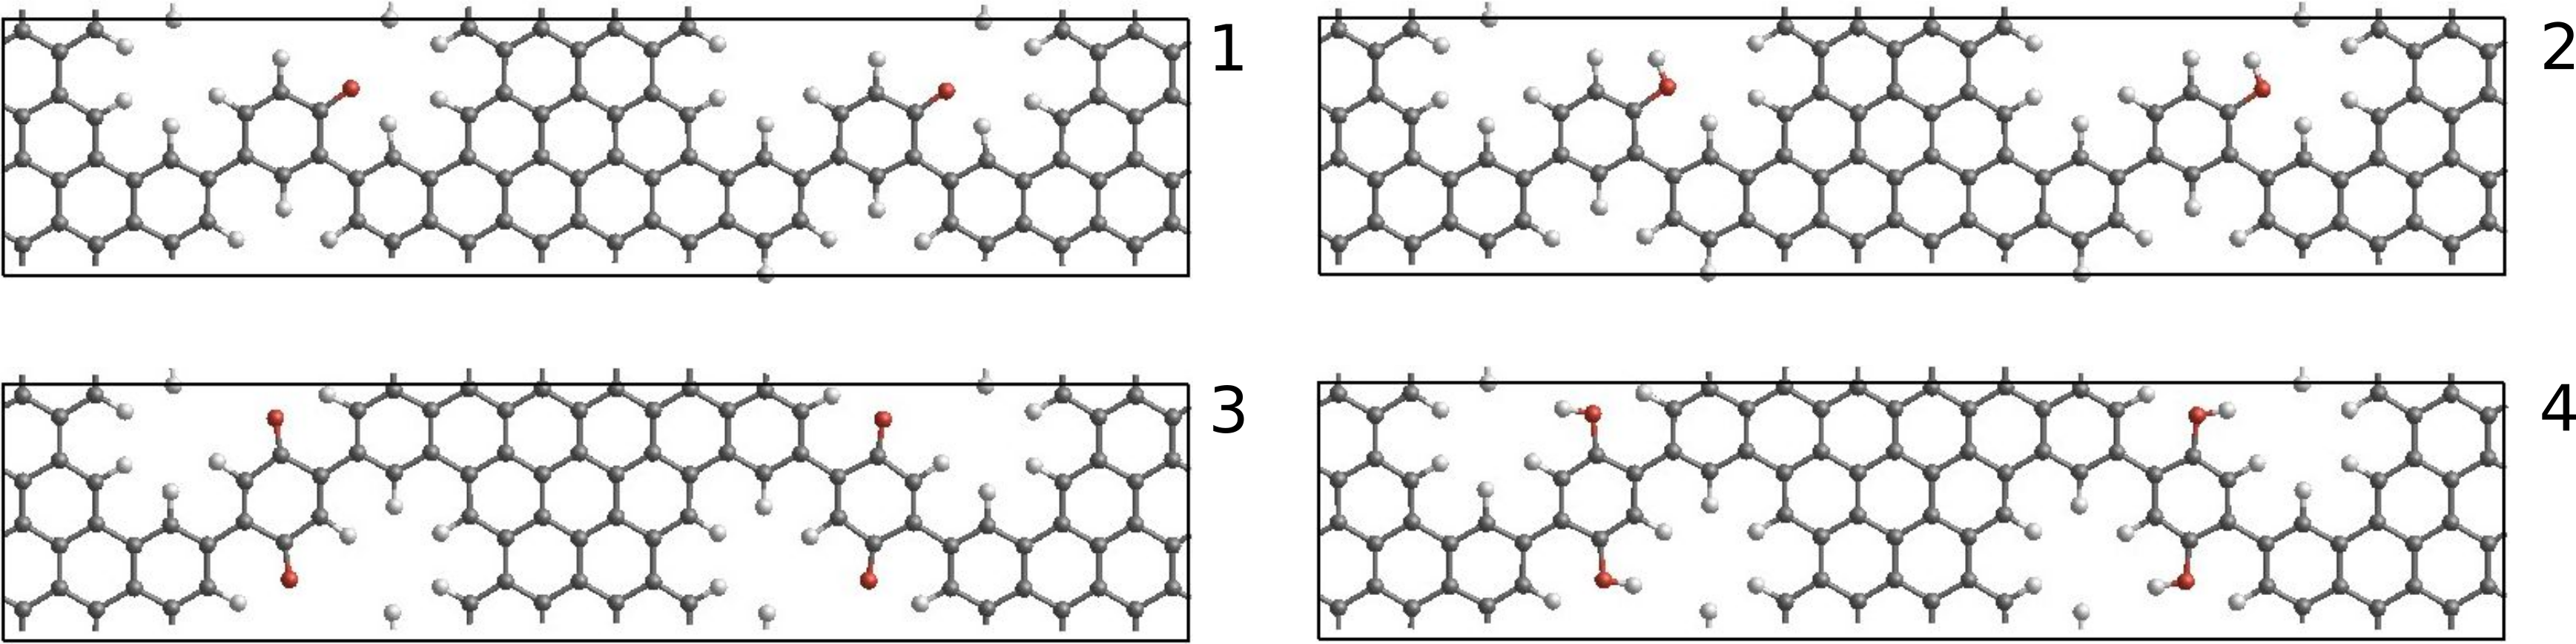
\includegraphics[width=\textwidth]{Figures/Structures.png}
	\caption{Figure showing all the structures stated in \cref{testtable}.}
	\label{Strucow}
\end{figure}

\im{Listings/Functions.py}{245}{252}
\vspace{-1\baselineskip}
\captionof{listing}{Code piece showing how the periodic Hamiltonian, shifted in the transverse direction i created using the given unit vector in the y direction.}{\label{periodichamilcode}}\vspace{\baselineskip}

\im{Listings/Functions.py}{234}{242}
\vspace{-1\baselineskip}
\captionof{listing}{Code piece showing how the transmission per energy point, using equation \cref{transeq}}{\label{transmissioncode}\vspace{\baselineskip}

% \section{Project overview}
% A Gantt chart is provided on the next page. \textbf{Not Updated.}
% \newpage
% \begin{turnpage}
% \setcounter{myWeekNum}{6}
% \ganttset{%
% 	calendar week text={\myWeek{}}%
% }
% \begin{figure}\vspace{-10mm}
% \begin{ganttchart}[
% 		hgrid,
% 		vgrid={*{6}{draw=none}, dotted},
% 		x unit=.15cm,
% 		%	y unit title=.6cm,
% 		%	y unit chart=.6cm,
% 		inline,
% 		milestone inline label node/.append style={left=5mm},
% 		milestone/.append style={xscale=3},
% 		time slot format=isodate,
% 		time slot format/start date=2019-02-04
% 	]{2019-02-04}{2019-05-31}
% 	\gantttitlecalendar{year, month=shortname, week}\\
% 	\ganttgroup{Report writing}{2019-02-25}{2019-05-31}\\
% 	\ganttgroup[inline = false]{Course 33442}{2019-02-04}{2019-03-31}\\
% 	\ganttbar{Ch. 1 \& 2}{2019-02-04}{2019-02-17}\\
% 	\ganttlinkedbar[link bulge=2]{Ch. 3}{2019-02-18}{2019-02-24}\\
% 	\ganttlinkedbar[link bulge=2,bar inline label node/.style={right=15pt}]{Ch. 4 \& 5}{2019-02-25}{2019-03-03}\\
% 	\ganttgroup[inline = false]{Python code}{2019-03-04}{2019-03-31}\\
% 	\ganttbar{Py TB scripts}{2019-02-18}{2019-03-17}\\
% 	\ganttlinkedbar[link bulge=2, bar inline label node/.style={right=45pt}]{Small NPG systems simulations}{2019-03-10}{2019-03-31}\\
% 	\ganttmilestone{Proof of Concept with Python}{2019-03-31}\\
% 	\ganttgroup[inline = false]{Large scale TB}{2019-04-01}{2019-04-28}\\
% 	\ganttbar[bar inline label node/.style={left=10pt}]{SISL \& TBtrans tutorial}{2019-04-01}{2019-04-05}\\
% 	\ganttlinkedbar[link bulge=2, bar inline label node/.style={right=50pt}]{Setup NPG variations}{2019-04-06}{2019-04-28}\\
% 	\ganttgroup[inline = false]{Generate data}{2019-04-28}{2019-05-31}\\
% 	\ganttmilestone{Hand in report}{2019-05-31}
% \end{ganttchart}
% \end{figure}
% \end{turnpage}
% \clearpage
% \global\pdfpageattr\expandafter{\the\pdfpageattr/Rotate 90}
